\SubProblem
{تابع درایور برنامه و آرگومان‌ها}
{
\begin{figure}[H]
    \centering
    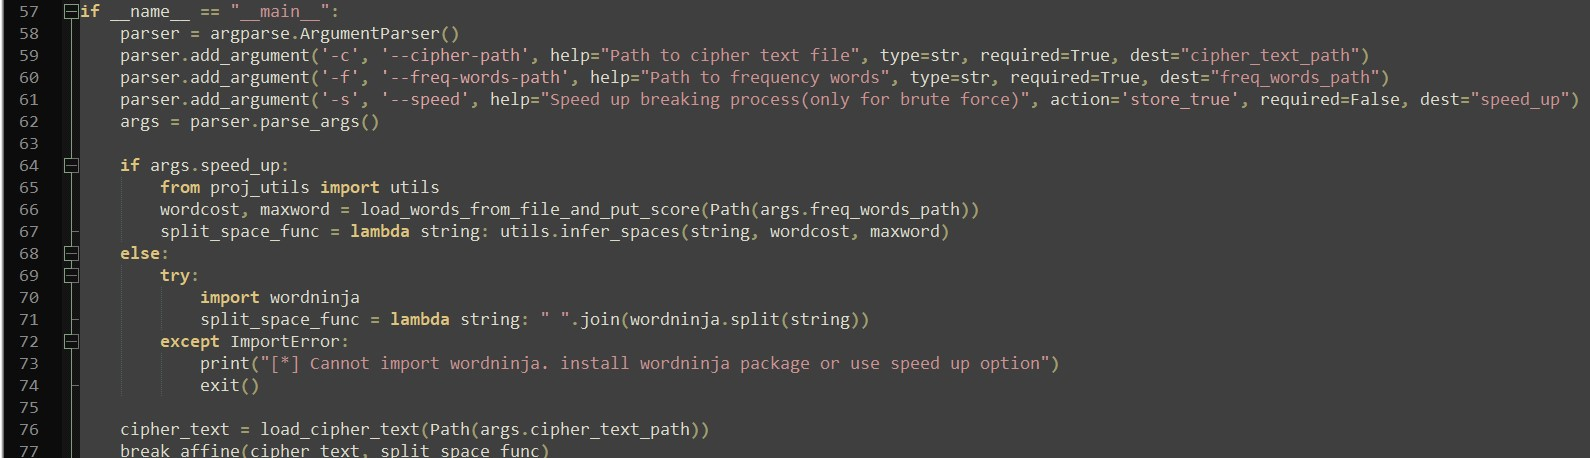
\includegraphics[width=15cm]{Images/F5.jpg}
    \label{fig:label}
    \caption{درایور برنامه و آرگومان‌ها}
\end{figure}

در این قسمت آرگومان‌های برنامه تعریف می‌شوند تا بر اساس آن‌ها برنامه راهنمای اجرا نیز داشته باشد. بر اساس پرچم
\lr{-s}
مشخص می‌شود اسپیس گذاری به چه نحوی صورت بگیرد.
دو روش برای فاصله گذاری ایجاد شده.

\begin{enumerate}
    \item
    استفاده از فایل فرکانس کلمات که روش سریع‌تری با دقت کمتر است.
    
    \item
    استفاده از کتابخانه
    \lr{wordninja}
    که روشی دقیق‌تر اما آهسته‌تری است.
    برای این روش شما باید این کتابخانه را نصب داشته باشید.
\end{enumerate}
}
